% Fiona Pigott
% March 2014

\documentclass[12pt]{article}
\usepackage[margin=1in]{geometry}
\usepackage{amsmath}
\usepackage{amssymb}
\usepackage{graphicx}
\usepackage{float}
\usepackage{multirow}
\usepackage{caption}
\usepackage{subcaption}
\usepackage[T1]{fontenc}
\usepackage{titling}


\setlength{\droptitle}{-3em} 

\title{DRAFT \\ Graph Metrics for Social Contagion \\ Data Analysis and Methods}
\author{Fiona Pigott}

\begin{document}


%Title
\maketitle

\section{Data treatment}

\subsection{Social network data}

The social network of this data set consists of phone number nodes (presumably corresponding to households or people) and phone call edges. The raw data lists of total phone calls between nodes in a given month for a span of ten years (from 1998 to 2007). These lists are directed (A calls B is different from B calls A) and aggregated monthly (all of the minutes of calls from A to B in one month are summed). The graphs (adjacency matrices) created from these lists are weighted and directed.

Before any analysis is performed, the graphs are made undirected (A calls B is equivalent to B calls A) in the following way. If the relationship between two nodes is mutual in a given month (A calls B and B calls A), the total number of calls are summed, and that total is the weight of the edge between A and B. If the relationship between two nodes is not mutual in a given month (A calls B, but B does not call A), the edge is removed from the graph. Approximately 57\% of the edges are removed from the graph in this step.

Most of the analysis in this paper makes use of an unweighted version of the graph, which is the same graph with all edge weights equal to one.

Note that after the above treatment, only about 2/3 of the listed nodes are participating in the network at any given time. Because this is a significant percentage, corrections are made to remove non-participating nodes from relevant calculations.

\subsection{Adoption data}
Raw infection data is given as a matrix with dimension (nodes) X (time steps), where if a node has internet service in a given month, that entry is equal to one and no internet service is denoted by a zero. Until 2003 the only internet service available was dial-up, and even after 2003 dial up was the most common form of internet service. Dial-up only charges per connection, so a user that begins using internet may not use it every month afterwords. This fluctuation between \(1 \rightarrow 0 \rightarrow 1\) is common in the time series, and accounted for by treating \(0\) users as susceptible entities.

\subsection{Anomalies and exclusions}
In the months April 2004 and October 2007, the total weights of phone calls (edges) dropped almost to zero from more than \(10^4\), removing almost all links between nodes on the graph. The total number of internet adopters also dropped to almost zero. The data for these months has been removed for the purpose of this analysis.

February 2001 has approximately the same number of edges and weights in the graph (number of links/ calls), but it has almost no correlation with any other graph in the time series, almost as if all of the links have been randomly scrambled. This month has been excluded from the data set for the purpose of analysis.

In the months May 2004 and November 2007, while the number of links between nodes on the graph does not seem to change drastically, the total weight of the graph spikes to approximately double the total in any other month. Because this analysis largely deals with the unweighted graph these data sets are still used.

\section{Adoption over time}

Metrics showing adoption, or ``infection," over time. A first time adoption is the first time a node adopts, and each node can nay appear once in calculation involving first time adoptions. Generally, adoption only means a \(0 \rightarrow 1\) transition, and a node can transition more than once.

\begin{figure}[H]
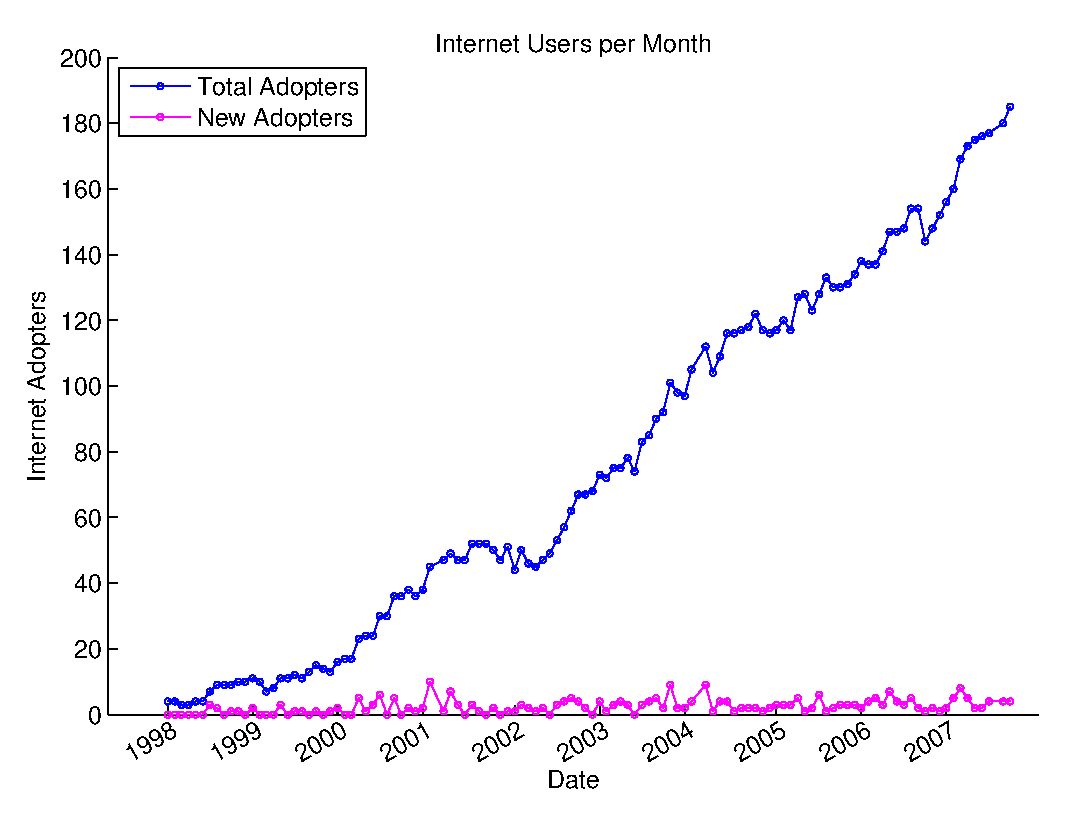
\includegraphics[width = .7\textwidth]{Graficos/AdoptersperMonth.eps}
\caption{Plot showing the number of adopters per month. Note that the number of new adopters per month does not change greatly and the number of total adopters grows linearly.}
\label{fig:AdoptersperMonth}
\end{figure}

\begin{figure}[H]
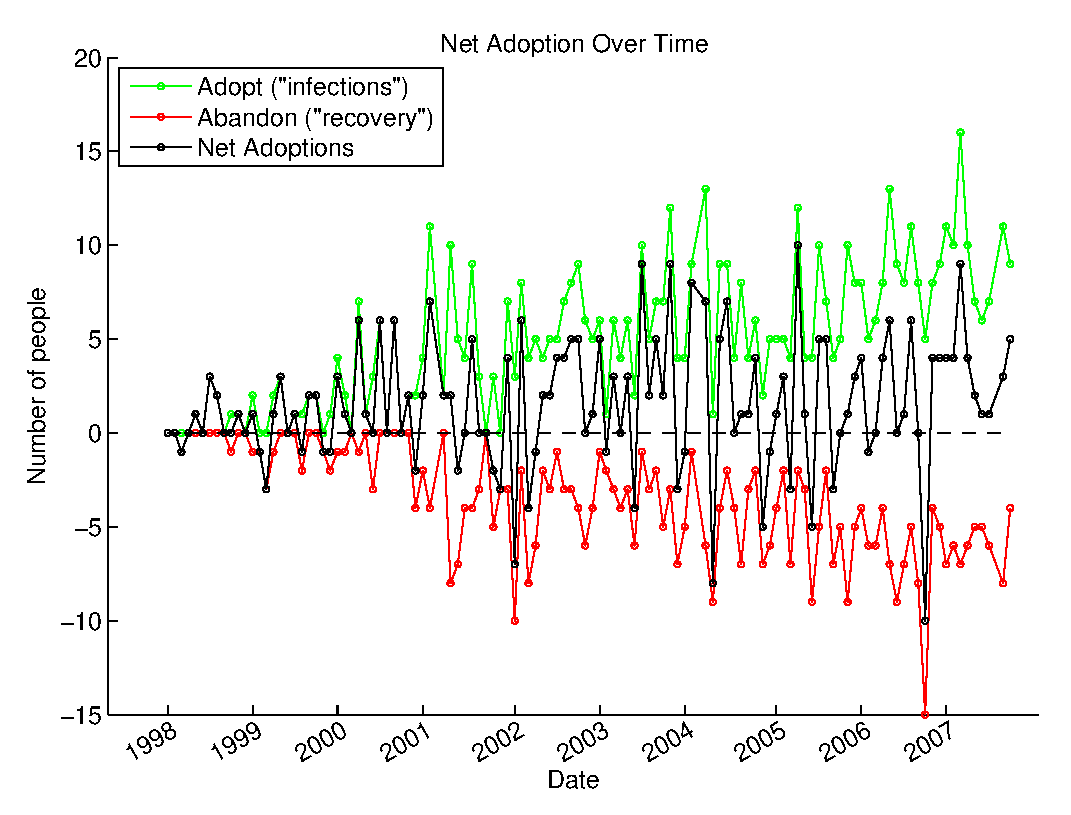
\includegraphics[width = .7\textwidth]{Graficos/trans.eps}
\caption{Fluctuations per month. Green shows the number of people who transition from susceptible to infected (S \(\rightarrow\) I), red the number of people who transition from infected to recovered (I \(\rightarrow\) R), and black the net change in the total number of adoptions for the given month.}
\label{fig:trans}
\end{figure}

\section{Topology of the social network over time}

\subsection{Neighborhood topological overlap}

To asses the changes between temporally adjacent graphs in the time-evolving network, we measure the topological overlap between graphs in the time series. We use a variation on the temporal correlation coefficient presented in \cite{3}, where our variation corrects for the large number of temporally disconnected nodes in the time series.

As defined in \cite{3}  the \emph{topological overlap} in the neighborhood of \(i\) between two consecutive time steps \([t_m,t_{m+1}]\) as:
\begin{equation}
C_i(t_m,t_{m+1}) = \frac{ \sum_j a_{ij}(t_m)a_{ij}(t_{m+1})}{\sqrt{[ \sum_j a_{ij}(t_m)][ \sum_j a_{ij}(t_{m+1})]}}
\label{eq:Ci}
\end{equation}

where \(a_{ij}\) represents an entry in the unweighted adjacency matrix of the graph, so summing over \(a_{ij}\) gives the edges between \(i\) and every other node.

Then the \emph{average topological overlap} of the graph at \(t_m\) with the subsequent graph at \(t_{m+1}\) is given by:

\begin{equation}
C_m = \frac{1}{\max [N(t_m),N(t_{m+1})]} \sum_{i = 1}^{N} C_i(t_m,t_{m+1})
\label{eq:Cm2}
\end{equation}

Here, we average by the maximum number of nodes participating in the network, instead of the total number of possible participating nodes. The metric presented by \cite{3} averages by a fixed \(N\), the total number of nodes in the network, and thus gives a value that underestimates the topological overlap by the percentage of non-participating nodes.

And the average temporal overlap between any two temporally adjacent graphs (the \emph{temporal correlation coefficient}) in the series is given by:

\begin{equation}
C = \frac{1}{M-1}\sum_{m=1}^{M-1}  \left( \frac{1}{\max [N(t_m),N(t_{m+1})]} \sum_{i = 1}^{N} C_i(t_m,t_{m+1}) \right)
\label{eq:C2}
\end{equation}

For this time series, the temporal correlation coefficient is 0.5282. Note that using the metric in \cite{3}, the temporal correlation coefficient result is 0.3834.

\begin{figure}[H]
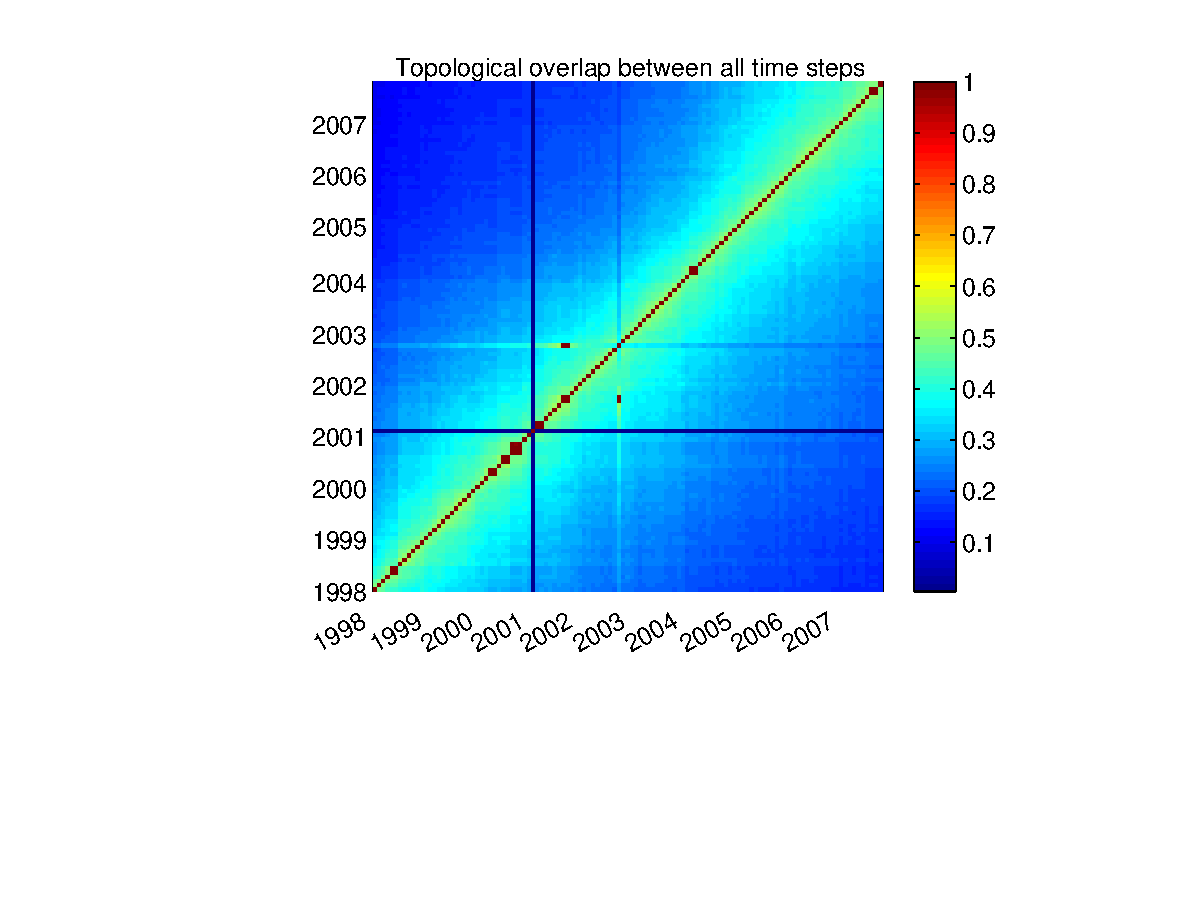
\includegraphics[trim = 0cm 0cm 0cm 0cm, width = .9\textwidth]{Graficos/overlap.eps}
\label{fig:overlap}
\caption{From the temporal correlation data, we can see that as time passes, the global changes in the graph progress evenly. That is, the graphs do not change more in the beginning than at the end of the observed window (the gradient from red to navy is not greater at the bottom left than the top right). We can also see that as time progresses the global features of the graphs overlap less and less. On average the topological overlap between a graph and its temporal neighbor is 0.5282, the temporal correlation coefficient. Between any two graphs, the average overlap is 0.2836, and between the two most separated graphs (the first and the last) the topological overlap drops to 0.1099, which can be said to be the stable kernel of the series. \newline However, that these figures only speak to global tendencies. Each neighborhood of each node changes differently, at a different rate and with significant monthly fluctuations, and it is interesting to note that every node \(i\) has at least one point where the temporal overlap between the neighborhood of \(i_m\) and \(i_{m+1}\) is equal to zero.}
\end{figure}



\subsection{Graph characteristics}

\begin{figure}[H]
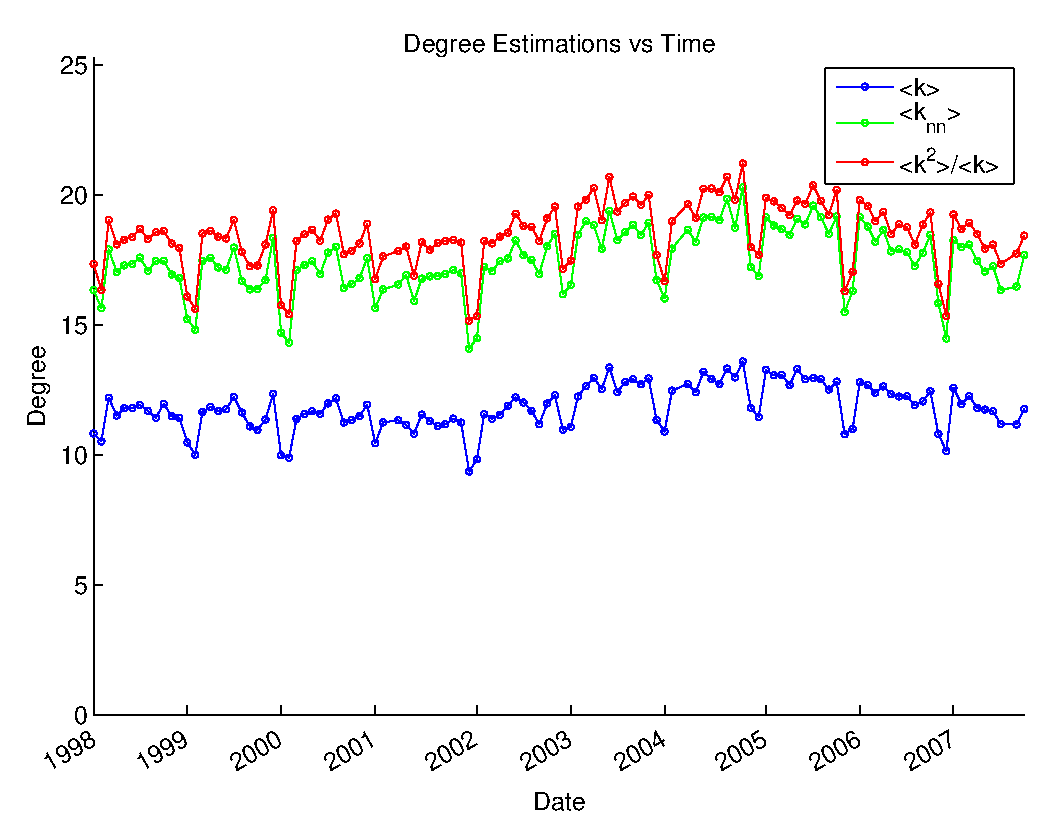
\includegraphics[trim = 0cm 0cm 0cm 0cm, width = .9\textwidth]{Graficos/NearestNeighbors.eps}
\label{fig:k}
\caption{Average degree and degree estimations over time, taken over participating nodes only (to correct for the fact that the number of participating nodes increases over time). }
\label{fig:nn}
\end{figure}

\subsubsection*{Degree, \(k\):}

The average degree of the participating nodes in the graph maintains relatively constant (a line of best fit has a slope of \(0.01\)). Further, variation between months is much less than variation between nodes: the sample standard deviation of the average degree (of participating nodes) between months is \(0.85\), while the standard deviation of the average degree over all months between nodes is \(7.32\). Individual nodes, however, do show significant variation in degree over time, changing between participating and non-participating, and also varying degree.

\subsubsection*{Nearest neighbor degree, \(k_{nn}\):}

The average degree of the nearest neighbors of participating nodes. 

\subsubsection*{\(k_{nn}\) estimation, \(\frac{<k^2>}{<k>}\):}

For non-assortative graphs, \(k_{nn} = \frac{<k^2>}{<k>}\).
For \(K\), a random variable taking the value of the degree of a node in the graph, the probability distribution of degree is the function \(P(K = k)\).
\[<k> = \sum_k kP_k\]
The probability of a node with degree \(k\) having a neighbor with degree \(h\): \( = q(H = h | K = k)\)
%And the average degree of nearest neighbors of a node with degree \(k\) is:
%\[k_{nn}(k) = \sum_h hP(H = h| K = k)\]
Which is the probability of following a random link from a node with degree \(K\) to a node with degree \(H\), given that \(K = k\). Now, if  the graph is non-assortative, that is, nodes are no more or less likely to connect with other nodes of the same degree, \(H = h\) and \(K = k\) are independent events and the distribution of \(q\) is independent of \(k\) and can be simplified further:
\[ q(H = h | K = k) = \frac{ k P(H = h)}{<k>}\]
%And then summing over \(k\) gives the distribution of nearest neighbor degree on the graph, independent of \(k\):
%\[ k_{nn}(k) = \sum_k q(H = h | K = k) = \sum_k \frac{P(H = h) P(K = k)}{P(K = k)}  = \]
Then, recognizing that \(H\) and \(K\) are identically distributed random variables of node degree, the average value of \(k_{nn}\) on the graph is the expected value of the function \(k_{nn}(k)\):
\[<k_{nn}> = \sum_{k} \frac{ h P(H = h)}{<k>} =  \frac{<k^2>}{<k>}  \]

On the social network, we can see that \(\frac{<k^2>}{<k>} \approx k_{nn}\), which is good evidence that the graph is non-assortative for degree.

\subsubsection*{Strength}

\begin{figure}[H]
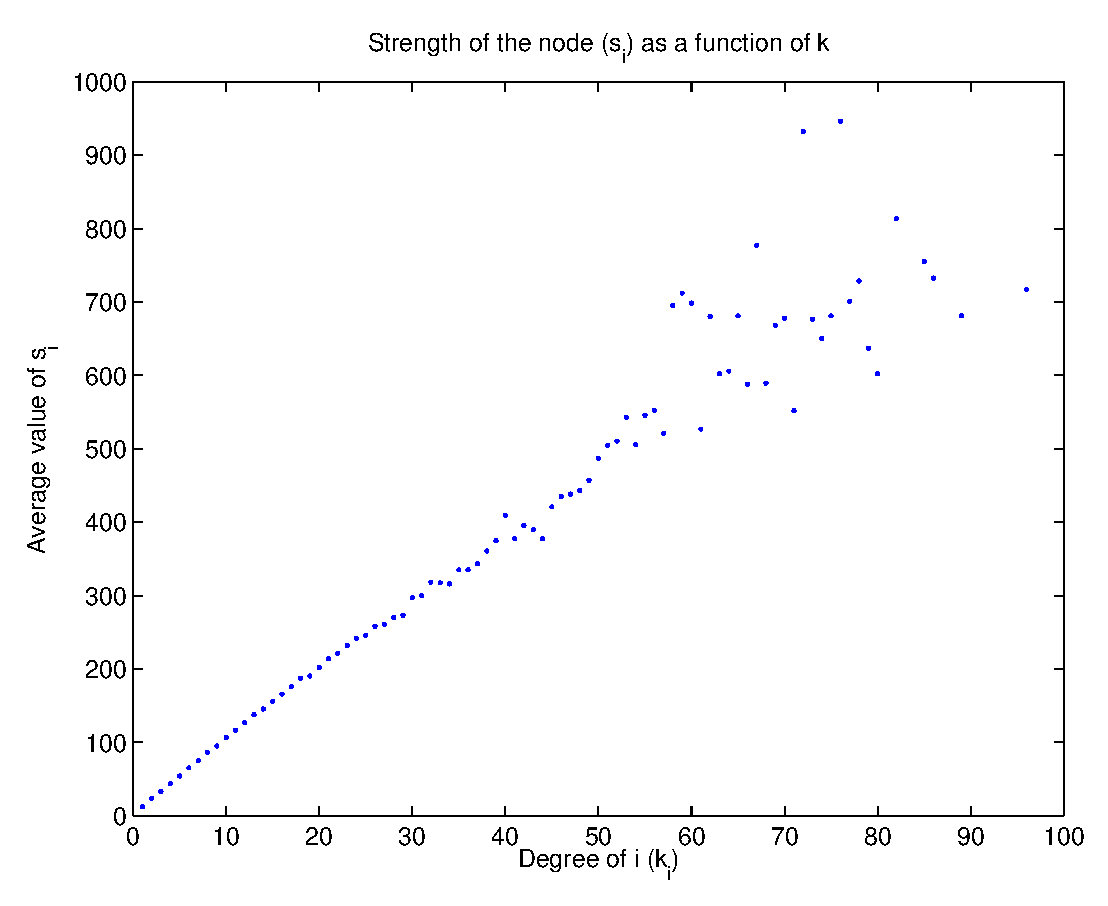
\includegraphics[trim = 0cm 0cm 0cm 0cm, width = .9\textwidth]{Graficos/svsk.eps}
\label{fig:svsk}
\caption{The data set used to construct these graphs also contains weight information (the number of times per month two phone number nodes call each other), but this analysis largely ignores edge weights (and node strength), instead simply using degree. The degree of a node can be used interchangeably with strength in this system, because \(k\) (degree, or the total number of edges of the node) is linearly related to \(s\) (strength, or the total weight of all edges of the node). This means that a node with many edges has the same average weight per edge as a node with very few edges. Indeed, the average weight of an edge on in the graph is \(10.3 \frac{calls}{connection}\), while the approximate slope of this line is \(9.9  \frac{calls}{connection}\). Larger deviation from this line for large \(k\) can likely be attributed to the fact that there are very few data points with very high degree.}
\end{figure}

\subsubsection*{Degree assortativity:}

%\begin{figure}[H]
%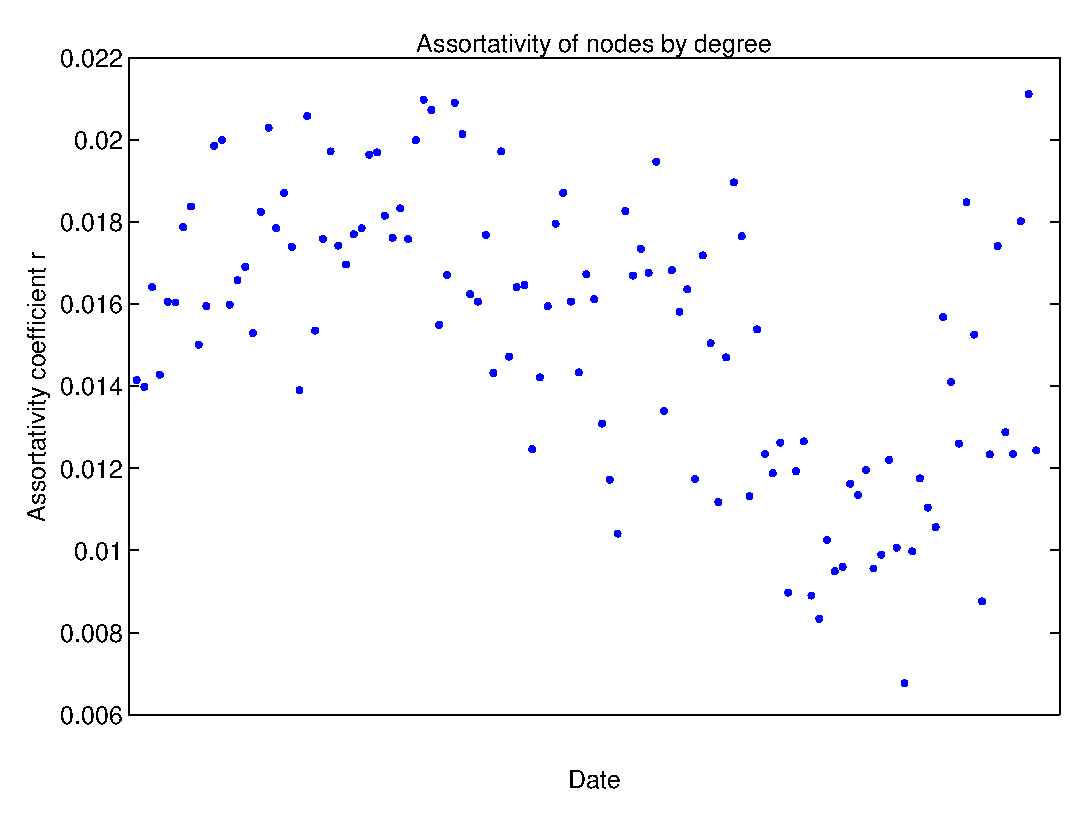
\includegraphics[trim = 0cm 0cm 0cm 0cm, width = .9\textwidth]{Graficos/degreeAssort.eps}
%\label{fig:degreeAssort}
%\caption{Degree assortative of the graph is the tendency for nodes to relate to other nodes with similar (or different) degree. High assortativity (\(r \approx 1\)) means that nodes relate largely to other nodes with the same degree. Conversely, (\(r \approx -1\)) means that nodes relate to other nodes with very different degree (high degree nodes relate to low degree ones). In }
%\end{figure}

Degree assortativity of a graph is the tendency for nodes to relate to other nodes with similar (or different) degree. High assortativity (\(r \approx 1\)) means that nodes relate largely to other nodes with the same degree. Conversely, low assortativity (\(r \approx -1\)) means that nodes relate to other nodes with very different degree (high degree nodes relate to low degree ones). 

Assortativity can be measured as the Pearson correlation coefficient \(r\), where \(q\) is the degree distribution of a vertex at the end of a randomly chosen edge (i.e., degree distribution of nearest neighbors, as described above), \(\sigma^2_q\) is the sample variance of \(q\) and \(e_{jk}\) is the joint probability distribution of the degrees of two connected vertices \cite{2}.

\begin{equation}
r = \frac{1}{\sigma^2_q} \sum_{jk} jk(e_{jk} - q_{j}q_{k})
\label{eq:rk}
\end{equation}

 Practically, this metric is evaluated as:
\begin{equation}
r = \frac{M^{-1} \sum_i j_i k_i - [M^{-1} \sum_i \frac{1}{2} (j_i + k_i)]^2}{M^{-1} \sum_i\frac{1}{2} (j_i^2 + k_i^2) - [M^{-1} \sum_i \frac{1}{2} (j_i + k_i)]^2}
\end{equation}

For a network with no assortative mixing, \(q_j\) an d\(q_k\) are independent, and \(e_{jk} = q_{j}q_{k}\), so the coefficient is identically zero. In the case of this network, degree assortativity ranges from \( 0.0068 \) to \(0.0211\), a showing once again that we can estimate the social network as a non-assortative graph.

\subsubsection*{Degree distribution}

\begin{figure}[H]
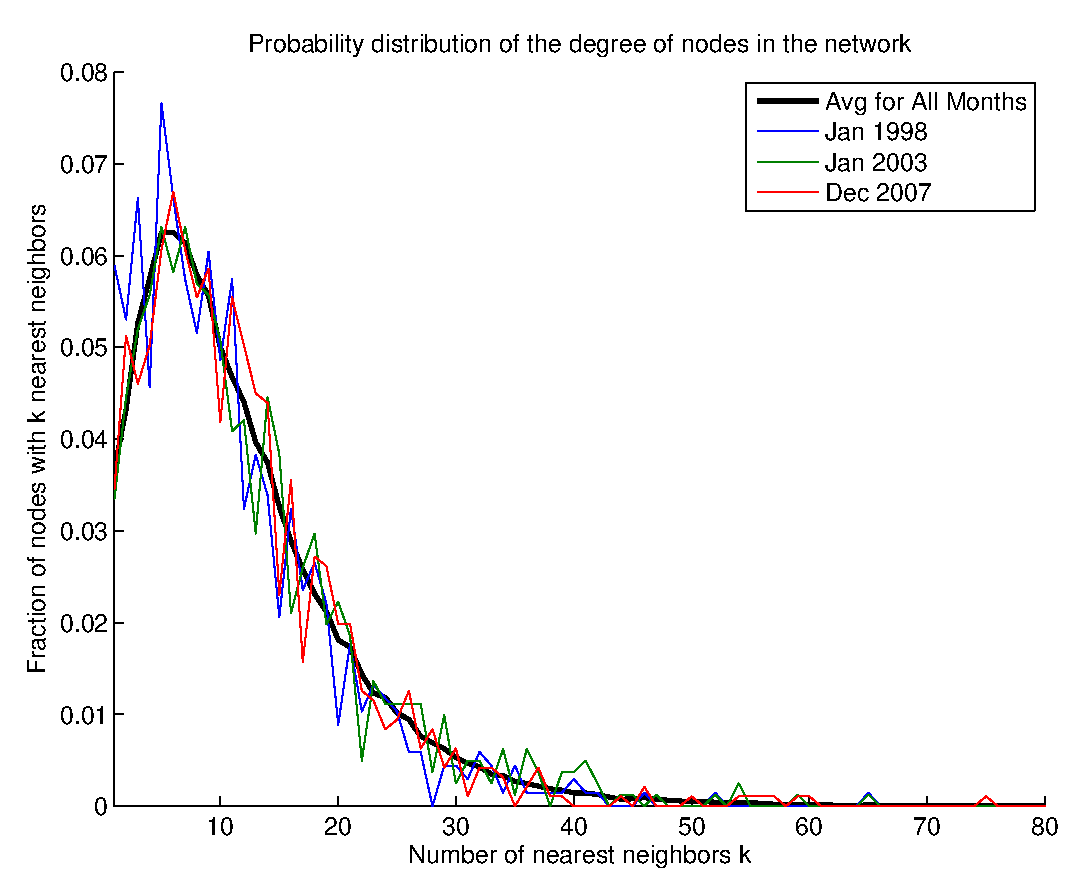
\includegraphics[trim = 0cm 0cm 0cm 0cm, width = .9\textwidth]{Graficos/ProbDistk.eps}
\label{fig:ProbDistk}
\caption{Because degree variation between time steps is small compared to degree variation between nodes (see fig \ref{fig:nn}) and we can see that the distribution of degree over the months remains roughly the same, it is possible to estimate the probability distribution of degree as the average of the probability distribution of degree in each month. This is convenient because it allows for comparison of node degree across months.}
\label{fig:Pk}
\end{figure}

\subsubsection*{Clustering}

A clustering coefficient can be used to show what fraction of the nodes in a graph are involved in triangles, or what the density of \emph{cliques} (sets of nodes where every node is connected to every other node) is in the graph.

\begin{figure}[H]
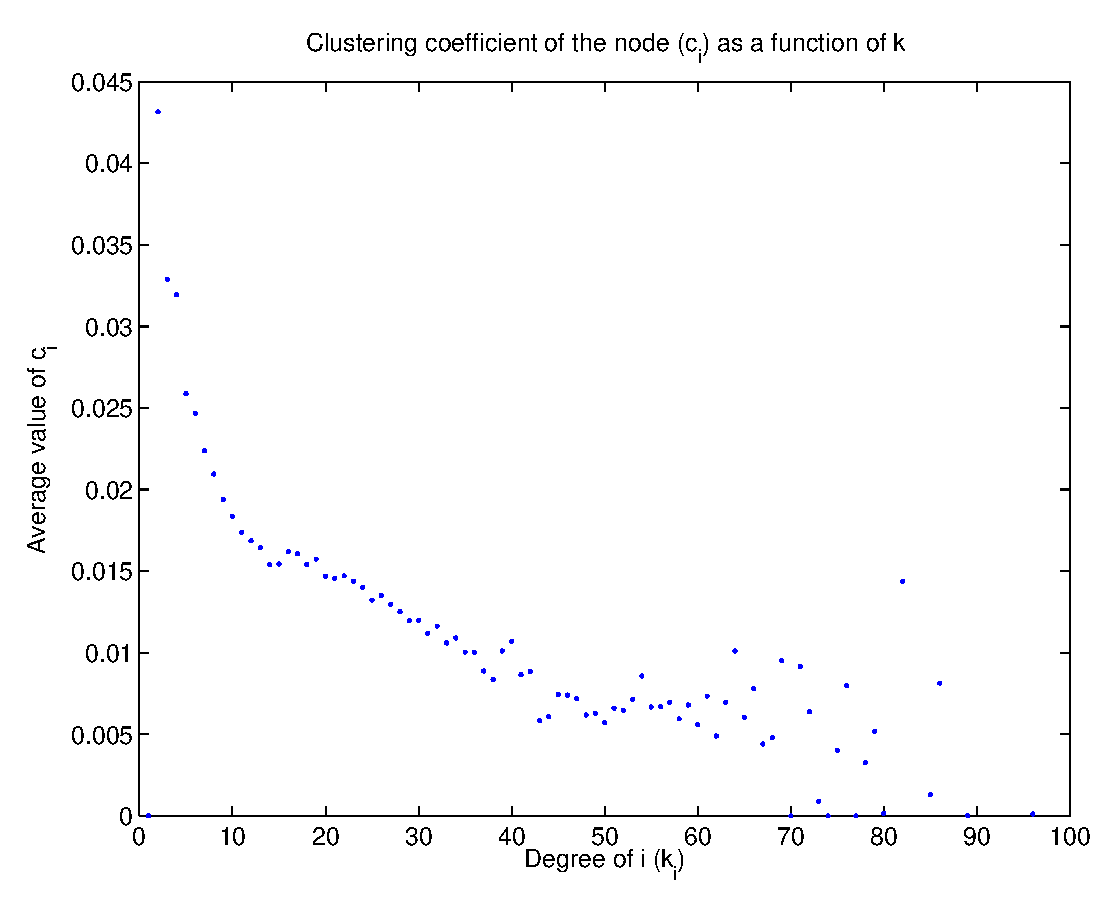
\includegraphics[trim = 0cm 0cm 0cm 0cm, width = .9\textwidth]{Graficos/clusteringcoeff.eps}
\label{fig:cluster}
\caption{The clustering coefficient in the social network is very low. This is possibly because while there are clusters in the graph there are few sets where every node is connected to every other. As the degree of the nodes involved decreases, so does the likelihood of every involved node being directly connected.}
\end{figure}

\section{Network topology and adoption}

\begin{figure}[H]
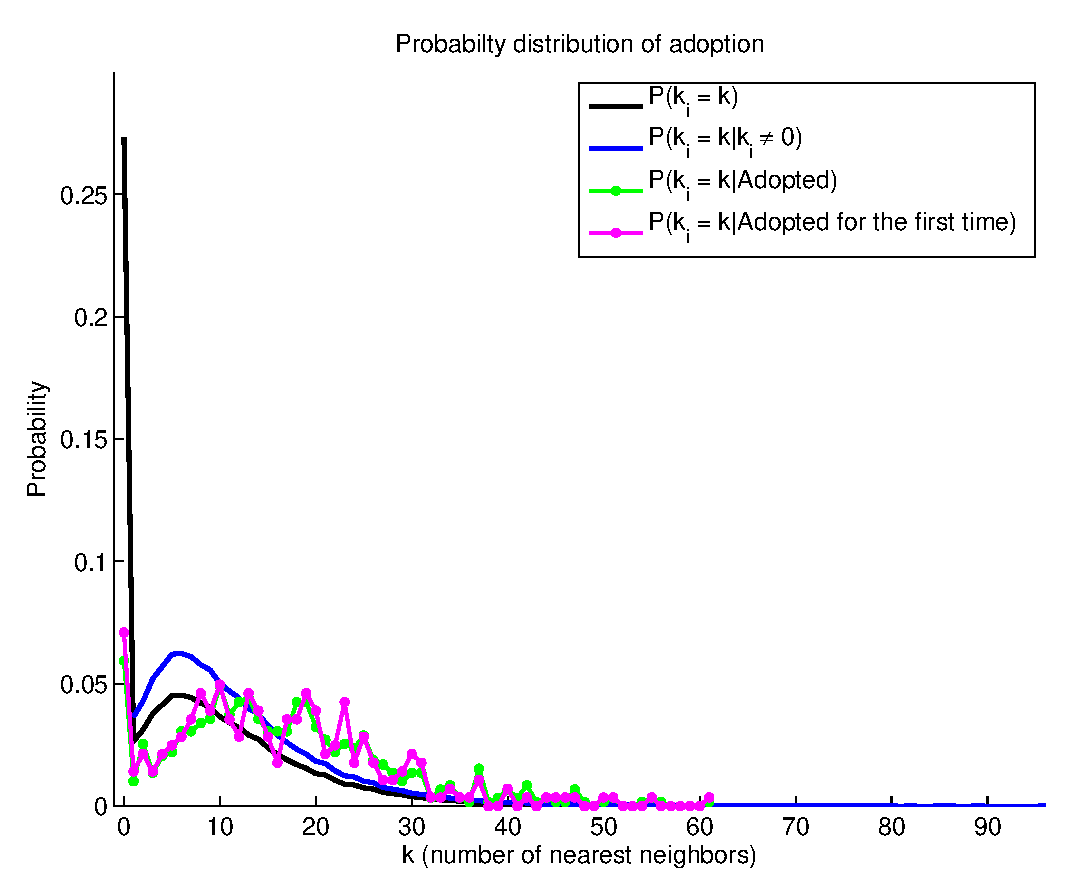
\includegraphics[trim = 0cm 0cm 0cm 0cm, width = .9\textwidth]{Graficos/PkGivenAdopt.eps}
\label{fig:PkGivenAdopt}
\caption{A comparison of the degree of an adopting node at the time of adoption, and the degree of all nodes in the network. We can see that an adopting node is likely to have a significantly higher degree than a non-adopting node: the mean degree of an adopting node is 17.2, while the mean degree of all nodes is 8.6 (for all nodes) or 11.8 (for only participating nodes). 85\% of all nodes and 80\% of participating nodes have less than the mean degree of an adopter (most, but not all,  adopters are participating nodes, so it is necessary to compare to both distributions of degree). That is to say, a group of adopters has a significantly higher degree than a randomly chosen group of nodes. \newline This comparison is meaningful for two reasons. One, the distribution of degree in general does not increase with time, so if the degree \(k_i\) of an adopting node \(i\) in some time step \(t_m\) is higher than average in \(t_m\) it can likely be said to be generally higher than average. Two, the network is not assortative for degree, so showing that adopters have generally higher degree does not simply mean that high degree nodes associate and are adopters.}
\label{fig:PkgA}
\end{figure}

\begin{figure}[H]
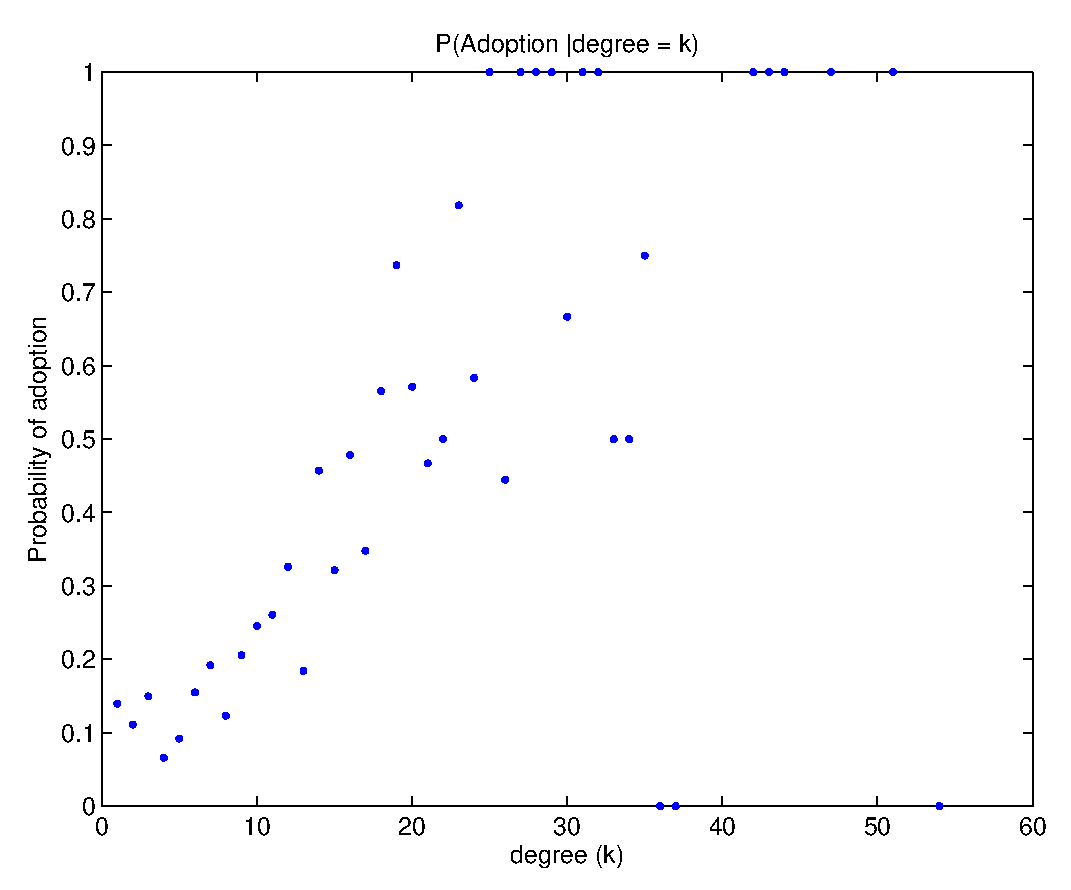
\includegraphics[trim = 0cm 0cm 0cm 0cm, width = .9\textwidth]{Graficos/ProbAgk.eps}
\label{fig:ProbAgk}
\caption{Fig (\ref{fig:PkgA}) gives the conditional probability \(P(K = k | Adopt)\) at the time of adoption, this figure gives \(P(Adopt | K = k)\), or the probability of the node adopting (first adoption only) when the degree is equal to \(k\). The same relationship holds in reverse: just as adopters have higher degree, nodes with a higher degree are more likely to be adopters. The probability that a node becomes an adopter at any time during the observed window is \(P(Adopt) = 0.25\), and it can be seen that nodes with a high degree are more likely to become adopters. For very high degree nodes probabilities are either 0 or 1 because there are only one or two data points for very high degrees.}
\end{figure}

Finally, we can discuss assortative mixing for any set of groups of nodes. In this case, we discuss assortative mixing of adopters in the network and define the \emph{assortativity coefficient} as:

\begin{equation}
r = \frac{\sum_i e_{ii} - \sum_i a_i b_i}{1 - \sum_i a_i b_i} = \frac{Tr \mathbf{e} - || \mathbf{e}^2||}{1 - || \mathbf{e}^2||}
\end{equation}

where \(e_{ij}\) is the fraction of edges connecting a node of type \(i\) (adopter) to a node of type \(j\) (non-adopter) and \(a_i\) and \(b_i\) are the fraction of each type of an end of an edge attached to a vertex of type \(i\). For perfectly assortative mixing \(r = 1\) and for non-assortative mixing \(r = 0\) \cite{1}.

\begin{figure}[H]
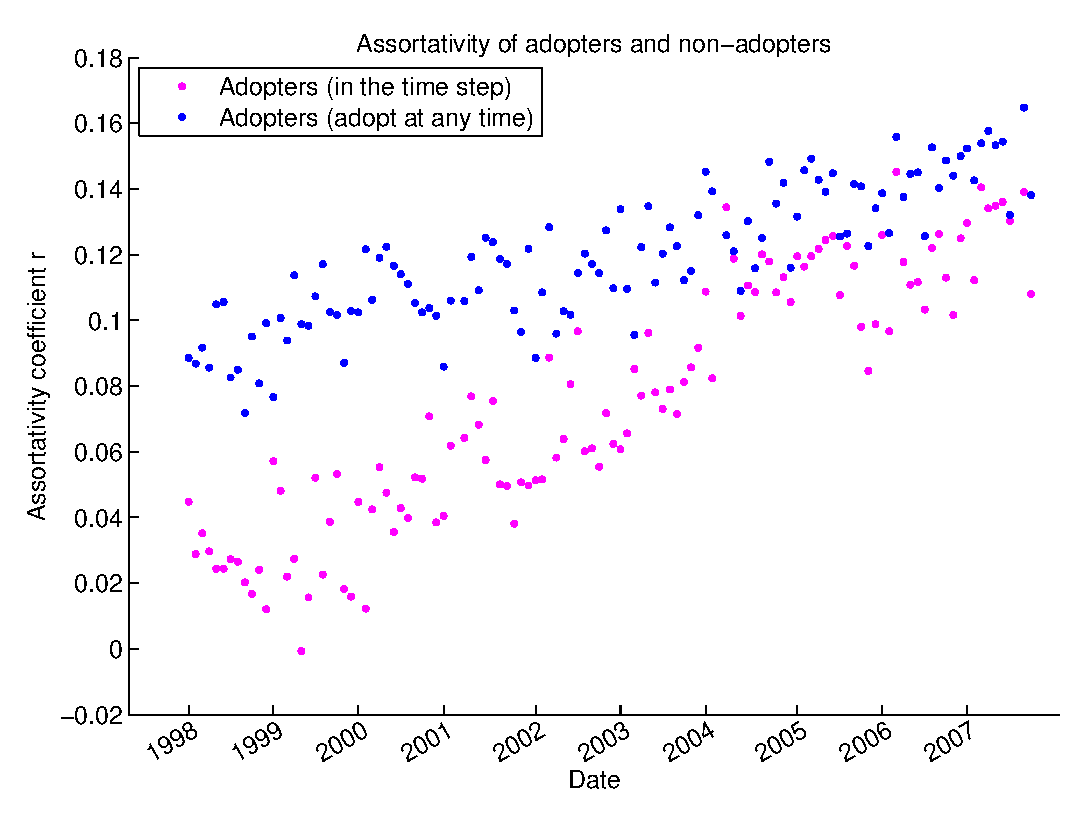
\includegraphics[trim = 0cm 0cm 0cm 0cm, width = .9\textwidth]{Graficos/adoptAssort.eps}
\label{fig:adoptAssort}
\caption{Assortative mixing of adopters in the social network. The series "Adopters (in the time step)" only looks at the assortativity of nodes who are currently adopters, while the series "Adopters (adopt at any time)" shows the assortativity of the group of people who, at some point, adopt. From this we can see that many adopters were connected well before adopting, and perhaps the group of people with the potential to adopt were previously connected for other reasons.}
\end{figure}


%
%you can, if you want, include network exposure with the proj method, but I won't recommend it
%
%lite vs heavy user (maybe)

\begin{thebibliography}{99}
\bibitem{1} M E J Newman. ``Assortative mixing in networks." 
\bibitem{2} M E J Newman. ``Mixing patterns in networks."
\bibitem{3} V Nicosia et al. ``Graph Metrics for Temporal Networks." 
\end{thebibliography}






\end{document}